\documentclass[a4paper, french, twoside]{article}
\usepackage[latin1]{inputenc}
\usepackage[T1]{fontenc}
\usepackage[french]{babel}
\usepackage{textcomp}		% pour afficher correctement l'apostrophe
\usepackage{lmodern}		% Pour changer le pack de police
\usepackage[a4paper,left=2cm,right=2cm,top=2cm,bottom=2cm]{geometry}
%\usepackage{libertine}
\usepackage{graphicx}

\setlength{\parindent}{0cm}
\setlength{\parskip}{1ex plus 0.5ex minus 0.2ex}
\newcommand{\hsp}{\hspace{20pt}}
\newcommand{\HRule}{\rule{\linewidth}{0.5mm}}

\begin{document}

\begin{titlepage}
	\begin{sffamily}
	\begin{center}

    	% Upper part of the page. The '~' is needed because \\
    	% only works if a paragraph has started.
    	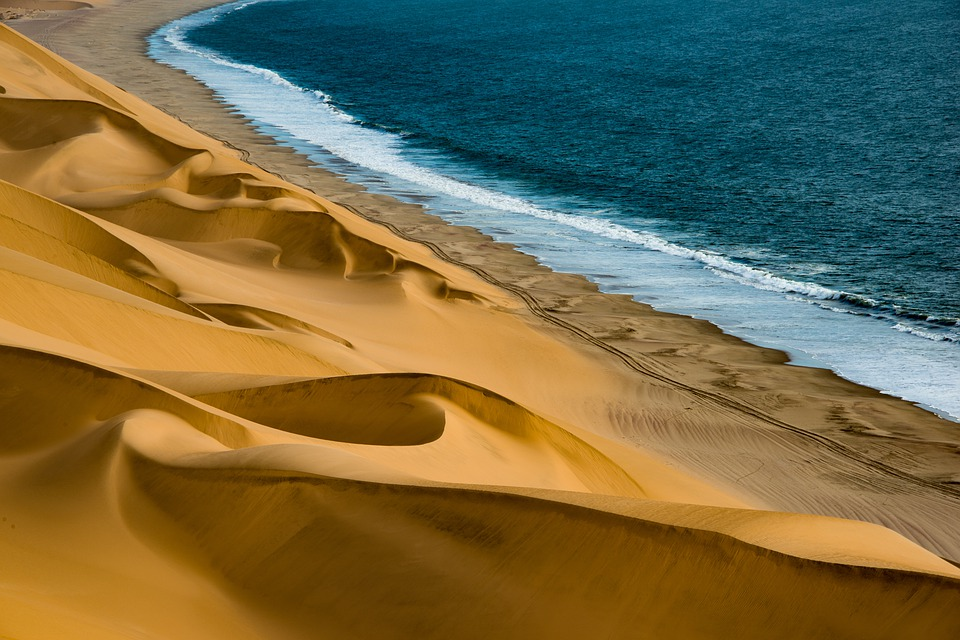
\includegraphics{IMAGES/dune.jpg}~\\[1.5cm]

    	\textsc{\LARGE �cole Sup�rieur d'�lectronique de Paris}\\[2cm]

    	\textsc{\Large TIPE 2\ieme ann�e}\\[1.5cm]

    	% Title
    	\HRule \\[0.4cm]
    	{ \huge \bfseries Mod�lisation d'�coulement granulaire\\[0.4cm] }

    	\HRule \\[2cm]
    	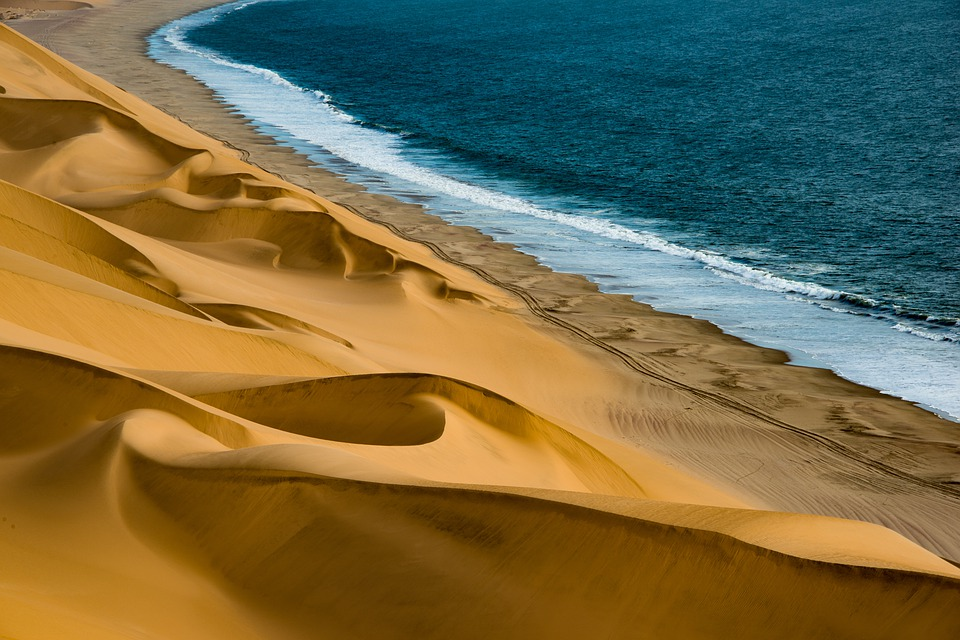
\includegraphics{IMAGES/dune.jpg}
    	\\[2cm]

    	% Author and supervisor
    	\begin{minipage}{0.4\textwidth}
      		\begin{flushleft} \large
			PARTENSKY Marc\\
        			COLIN Valentin\\
        			Promo 2023\\
     		 \end{flushleft}
    	\end{minipage}
    	\begin{minipage}{0.4\textwidth}
      		\begin{flushright} \large
        			\emph{Enseignant :} M. \textsc{SAINT-JALM} \\
			et M. \textsc{GAUDILLIERE}\\
			Sept 2019 - Juin 2020
     		 \end{flushright}
    	\end{minipage}

    	\vfill

    	% Bottom of the page
    	%{\large Septembre 2019 / Juin 2020}

  	\end{center}
 	\end{sffamily}
\end{titlepage}
\end{document}